%%
%% This is file `sample-sigconf.tex',
%% generated with the docstrip utility.
%%
%% The original source files were:
%%
%% samples.dtx  (with options: `all,proceedings,bibtex,sigconf')
%% 
%% IMPORTANT NOTICE:
%% 
%% For the copyright see the source file.
%% 
%% Any modified versions of this file must be renamed
%% with new filenames distinct from sample-sigconf.tex.
%% 
%% For distribution of the original source see the terms
%% for copying and modification in the file samples.dtx.
%% 
%% This generated file may be distributed as long as the
%% original source files, as listed above, are part of the
%% same distribution. (The sources need not necessarily be
%% in the same archive or directory.)
%%
%%
%% Commands for TeXCount
%TC:macro \cite [option:text,text]
%TC:macro \citep [option:text,text]
%TC:macro \citet [option:text,text]
%TC:envir table 0 1
%TC:envir table* 0 1
%TC:envir tabular [ignore] word
%TC:envir displaymath 0 word
%TC:envir math 0 word
%TC:envir comment 0 0
%%
%%
%% The first command in your LaTeX source must be the \documentclass
%% command.
%%
%% For submission and review of your manuscript please change the
%% command to \documentclass[manuscript, screen, review]{acmart}.
%%
%% When submitting camera ready or to TAPS, please change the command
%% to \documentclass[sigconf]{acmart} or whichever template is required
%% for your publication.
%%
%%
\documentclass[sigconf, screen, review]{acmart}

%%
%% \BibTeX command to typeset BibTeX logo in the docs
\AtBeginDocument{%
  \providecommand\BibTeX{{%
    Bib\TeX}}}

\usepackage{makecell}

%% Rights management information.  This information is sent to you
%% when you complete the rights form.  These commands have SAMPLE
%% values in them; it is your responsibility as an author to replace
%% the commands and values with those provided to you when you
%% complete the rights form.
\setcopyright{none} 
%\setcopyright{acmlicensed}
\copyrightyear{2026}
\acmYear{2026}
\acmDOI{XXXXXXX.XXXXXXX}

%% These commands are for a PROCEEDINGS abstract or paper.
\acmConference[MICRO 2026]{The 58th IEEE/ACM International Symposium on Microarchitecture}{October 31--November 04, 2026}{Athens, Greece}
%%
%%  Uncomment \acmBooktitle if the title of the proceedings is different
%%  from ``Proceedings of ...''!
%%
%%\acmBooktitle{Woodstock '18: ACM Symposium on Neural Gaze Detection,
%%  June 03--05, 2018, Woodstock, NY}

\acmISBN{978-X-XXXX-XXXX-X/XX/XX}


%%
%% Submission ID.
%% Use this when submitting an article to a sponsored event. You'll
%% receive a unique submission ID from the organizers
%% of the event, and this ID should be used as the parameter to this command.
%%\acmSubmissionID{123-A56-BU3}

%%
%% For managing citations, it is recommended to use bibliography
%% files in BibTeX format.
%%
%% You can then either use BibTeX with the ACM-Reference-Format style,
%% or BibLaTeX with the acmnumeric or acmauthoryear sytles, that include
%% support for advanced citation of software artefact from the
%% biblatex-software package, also separately available on CTAN.
%%
%% Look at the sample-*-biblatex.tex files for templates showcasing
%% the biblatex styles.
%%

%%
%% The majority of ACM publications use numbered citations and
%% references.  The command \citestyle{authoryear} switches to the
%% "author year" style.
%%
%% If you are preparing content for an event
%% sponsored by ACM SIGGRAPH, you must use the "author year" style of
%% citations and references.
%% Uncommenting
%% the next command will enable that style.
%%\citestyle{acmauthoryear}
\settopmatter{printfolios=true}
\settopmatter{printacmref=false}

\newcommand{\aj}[1]{{\color{cyan} AJ: {#1}}}
%\pagestyle{plain}

%%
%% end of the preamble, start of the body of the document source.
\begin{document}

%%
%% The "title" command has an optional parameter,
%% allowing the author to define a "short title" to be used in page headers.
\title{Guidelines for Submission to MICRO 2026}
\subtitle{\normalsize{MICRO 2026 Submission
    \textbf{\#NaN} -- Confidential Draft -- Do NOT Distribute!!}}
%%
%% The "author" command and its associated commands are used to define
%% the authors and their affiliations.
%% Of note is the shared affiliation of the first two authors, and the
%% "authornote" and "authornotemark" commands
%% used to denote shared contribution to the research.
\author{\normalsize{MICRO 2026 Submission
   \textbf{\#NaN} -- Confidential Draft -- Do NOT Distribute!!}}

%%
%% By default, the full list of authors will be used in the page
%% headers. Often, this list is too long, and will overlap
%% other information printed in the page headers. This command allows
%% the author to define a more concise list
%% of authors' names for this purpose.

%%
%% The abstract is a short summary of the work to be presented in the
%% article.

%%%%%% -- PAPER CONTENT STARTS-- %%%%%%%%


\begin{abstract}

Memory Dependence Prediction (MDP) is a speculative technique to determine which stores, if any, a given load will depend on. Area-constrained cores are increasingly relevant in various applications such as energy-efficient or edge systems, and can often only spare limited space for MDP tables. This leads to a high number of false dependencies as memory independent loads collide with unrelated predictor entries, causing unnecessary stalls. This paper proposes a profile-guided hardware/software co-design to detect frequently memory independent loads and labels them via their opcode to mark them as 'predict no dependency' (PND) loads. These PND loads bypass the MDP and are always scheduled as early as possible, eliminating the possibility of false dependencies without introducing additional hardware overhead. Across Spec2017 intspeed, this technique achieves a gmean IPC gain of 1.4\% in the smallest core simulated. On larger cores, performance is maintained while average MDP power usage is reduced by 40\%.

\end{abstract}
%%
%% The code below is generated by the tool at http://dl.acm.org/ccs.cfm.
%% Please copy and paste the code instead of the example below.
%%
%\begin{CCSXML}
%<ccs2012>
% <concept>
%  <concept_id>00000000.0000000.0000000</concept_id>
%  <concept_desc>Do Not Use This Code, Generate the Correct Terms for Your Paper</concept_desc>
%  <concept_significance>500</concept_significance>
% </concept>
% <concept>
%  %<concept_id>00000000.00000000.00000000</concept_id>
%  <concept_desc>Do Not Use This Code, Generate the Correct Terms for Your Paper</concept_desc>
%  <concept_significance>300</concept_significance>
% </concept>
% <concept>
%  %<concept_id>00000000.00000000.00000000</concept_id>
%  <concept_desc>Do Not Use This Code, Generate the Correct Terms for Your Paper</concept_desc>
%  <concept_significance>100</concept_significance>
% </concept>
% <concept>
 % <concept_id>00000000.00000000.00000000</concept_id>
%  <concept_desc>Do Not Use This Code, Generate the Correct Terms for Your Paper</concept_desc>
%  <concept_significance>100</concept_significance>
% </concept>
%</ccs2012>
%\end{CCSXML}

%\ccsdesc[500]{Do Not Use This Code~Generate the Correct Terms for Your Paper}
%\ccsdesc[300]{Do Not Use This Code~Generate the Correct Terms for Your Paper}
%\ccsdesc{Do Not Use This Code~Generate the Correct Terms for Your Paper}
%\ccsdesc[100]{Do Not Use This Code~Generate the Correct Terms for Your Paper}

%%
%% Keywords. The author(s) should pick words that accurately describe
%% the work being presented. Separate the keywords with commas.
\keywords{Do, Not, Use, This, Code, Put, the, Correct, Terms, for,
  Your, Paper}

\maketitle

\section{Introduction}

-turned into a false dependency/IPC story. is it still potentially worthwhile to try and push the MDP lookup reduction/predictor activity as a result? its only useful in so far as it reduces false deps (as percent power usage of MDP is so small), but maybe it could still be seen as interesting in its own right

Memory-level parallelism (MLP) is important for efficient out-of-order (OoO) execution and overcoming the memory wall in processor performance. Memory dependence prediction is a speculative technique used in OoO processors that aims to enhance total MLP by predicting the stores on which a given load instruction will depend, as well as identifying memory-independent loads. Smaller cores utilising smaller predictors can often struggle with a large number of false dependencies, which unnecessarily stalls loads on non-dependent stores. This is due to hash collisions in small predictor tables, or simple predictor algorithms that cannot capture varying dependency behaviour. The Store Sets predictor \cite{storesets} is exhibits both of these issues, and variations of the algorithm are found in real processors today \cite{openxiangshan}. Whereas modern predictors like PHAST \cite{phast} have pushed the SotA to address these issues via techniques like associative tagging and context based predictions, they place higher area, energy and complexity demands on core design, which is often not viable in smaller cores. At the same time, while simply growing a Store Sets-like predictor would offset the hash collisions, this benefit struggles to outperform an iso-area comparison to scaling other components. As such, memory dependence predictors in small cores typically remain small and inefficient.

At the same time, the importance of such area-constrained cores has grown over time. Modern systems increasingly deploy heterogeneous processors containing both performance and efficiency-oriented core designs, combining larger high-performance cores with small energy-efficient (but still out-of-order) cores, as seen in ARM big.LITTLE systems and both Apple’s \& Intel's performance and efficiency cores. Efficiency-focused cores are, of course, also found in power-constrained systems such as smartphones, tablets, smartwatches and other edge systems. These cores are more and more performing demanding general purpose computation while striving to consume as little energy as possible. As they grow more performance-sensitive, finding optimisations which don't also incur additional area, power or complexity costs becomes more pressing.

This paper builds on an observation demonstrated by various prior works that a considerable portion of load instructions in general-purpose workloads rarely or never exhibit in-flight memory dependencies \cite{store-distance,improving-mem-dep,constable}. This is exploited to reduce false dependencies in memory dependence prediction via a profile-guided software co-design at \textbf{zero hardware cost}. Our technique labels frequently memory-independent loads by their opcode, causing them to bypass MDP queries and always schedule as early as possible. We show that the vast majority of dynamic loads can avoid querying the MDP while maintaining or improving IPC, as well as provide a potential power saving.

\subsection{Contributions}
This paper makes the following contributions:
\begin{itemize}
        \item[$\bullet$] Implements a profile-guided co-design technique to label memory independent loads to the OoO core at no hardware overhead.
        \item[$\bullet$] Implements a modified Gem5 to simulate labelled loads against different MDP algorithms and core size configurations.
        \item[$\bullet$] Extends McPat to provide power usage estimations of the MDP unit.
        \item[$\bullet$] Evaluates Spec2017 IntSpeed and demonstrates on average: 
        \begin{itemize}
          \item[$\bullet$] IPC improves on the smallest core by 1.47\%,
          \item[$\bullet$] 71\% of MDP load queries are redundant,
          \item[$\bullet$] MDP power reduces by 12\% on the smallest core, whereas the largest core maintains IPC and reduces MDP power by 42\%. 
        \end{itemize}
        \item[$\bullet$] Additionally demonstrates a x\% IPC gain when modelling a limited number of MDP read ports.
        % \item[$\bullet$] (currently only includes 2 benchmarks) Evaluates Spec2017 FloatSpeed and demonstrates on average: 87\% of MDP load queries are redundant, IPC improves by 0.1\% \& MDP power reduces by 6.5\% on the smallest core, whereas the largest core maintains IPC and reduces MDP power by x\%. 
        % \begin{itemize}
        % \item[$\bullet$] Additionally demonstrates a 16.5\% IPC gain on highly constrained cores that lack any memory dependence prediction.
        % \item[$\bullet$] Additionally demonstrates a x\% IPC gain when modelling a limited number of MDP read ports.
        % \end{itemize}
\end{itemize}

\section{Background}

This section outlines the fundamental concepts in memory-level parallelism for out-of-order execution. It then introduces Store Sets as a foundational memory dependence predictor algorithm, a more modern variation found in the XiangShan processor, and lastly the current state of the art in the PHAST predictor.

\subsection{Loads in Out-of-Order Execution}
The key structure in memory-level parallelism is the load-store queue (LSQ), used to hold in-flight memory operations and perform memory disamgibuation. When load instructions dispatch, they are inserted into the load queue (LQ), and query the memory dependence predictor (MDP) for a predicted store(s) to wait on before execution. Once their source operands are ready and all predicted dependent stores have executed, loads search backwards through the store queue (SQ) for store-forwarding opportunities. If no matching addresses are found, the loads access cache to get their data.

When a load searches the SQ, not all earlier stores may have resolved their addresses. As the majority of the time the address will not match with the load, it is often profitable to speculatively ignore these stores and issue the load as soon as possible. When the unresolved store eventually receives it's address, it searches forward through the LQ to find loads with matching addresses which have already executed. If a match is found, the load has read stale data and a memory order violation has occured. The processor must flush all in-flight instructions from the load onwards and re-fetch.

The goal of the MDP is to minimise violation events while maximising the available MLP, allowing memory independent loads to issue as soon as possible and dependent loads to wait only for the necessary stores. When a load is incorrectly stalled on a store that does not resolve to the same address this is called a false dependency. Simple MDP algorithms typically prioritise reducing the number of violations over the number of false dependencies.

\subsection{Store Sets}
A seminal paper in memory dependence prediction is 'Memory Dependence Prediction using Store Sets' \cite{storesets}. This is the MDP algorithm implemented in the open source Gem5 simulator \cite{gem5}. Store Sets works by using Store Set IDs (SSID) to track dependent load-store pairs, assigning each instruction the same ID value in the PC-indexed Store Set ID Table (SSIT). The SSIDs are then used to index the Last-Fetched Store Table (LFST), which holds the sequence number of the most recently issued store with an SSID mapping to that LFST entry. Newly issued loads then access the LFST via their SSID to find the store they're predicted to be dependent on. If a load PC does not map to a valid SSID entry, it is predicted to be memory independent. To forget old dependencies and reduce table pressure, the SSIT and LFST are cyclically cleared after a certain number of issued memory operations.

Store Sets is extremely area efficient, delivering a large portion of available performance with a very small hardware budget. It's small size and simplicity make it well suited to area-constrained processors. However, especially at smaller sizes, Store Sets struggles with false dependencies due hash collisions. When a memory independent load hashes to an existing SSID entry, it is incorrectly made dependent on the corresponding store for that entry. The clear period can be made shorter to offset this, but this comes at the trade-off of a higher number of memory order violations as the predictor must re-learn true dependencies more often. Furthermore, many loads exhibit non-consistent memory dependencies. A load in a loop may be dependent on a store every even iteration, but not on odd iterations. Store Sets has no way to disambiguate these cases, and conservatively predicts the load as dependent on every iteration.

\subsection{XiangShan Store Sets}
XiangShan is an open-source high-performance RISCV processor RTL implementation \cite{xiangshan-paper}. XiangShan represents the cutting edge in open-source superscalar processor design, and comes with a Gem5 fork modified to closer model the RTL implementation \cite{xiangshan-gem5}. This Gem5 fork implements a variation of the Store Sets predictor that offers a closer representation to implementations found in real processors. From here on this is referred to as XS Store Sets.

The main optimisation over original Store Sets is using multiple 'slots' for each LFST entry, thereby recording multiple dependent stores at once. This allows a load to track multiple dependencies with only one SSID. This is useful in situations where a load is dependent on different stores in different program contexts, or may have partial address overlap with multiple stores. There are further small optimisations to allocation policy which we omit here.

\subsection{PHAST}
PHAST is a newer predictor which achieves much greater accuracy than Store Sets and other previously proposed MDP algorithms \cite{phast}. PHAST uses a TAGE-like structure to record a geometric series of branch history lengths between dependent load-store pairs. On dispatch, load instructions search all history length tables in parallel and selects the dependencies on the longest path (or predicts no dependency if no tables hit). This scheme addresses the previous problems in Store Sets by using multi-way tagged associative entries to reduce hash collisions, and predicting dependencies based on branch context to capture more elaborate dependency patterns. At a storage budget of 14.5KB, PHAST is shown to achieve within 1.5\% accuracy of an ideal predictor.

Although PHAST delivers much greater accuracy, it also comes with greater hardware overhead. Though PHAST greatly outperforms Store Sets for iso-area comparisons at larger budgets, it struggles with the smaller budgets most efficiency-focused cores allow for memory dependence prediction. Furthermore, PHAST incurs pipeline complexity by requiring global branch history be made available in the load-store unit, has greater prediction latency, and consumes more power for the same area. This makes PHAST better suited only for larger performance-focused cores that would benefit most from the greater MLP.

\section{Related Work}

- could copy constable's style of related work section by having a wide spray of references to loosely associated optimisation techniques. the literal hundreds of references is probably not needed though  \\
- should probably reference all the other MDPs

\subsubsection{Improving Memory Dependence Prediction with Static Analysis}
\cite{improvingmdp} tackles the same problem as this paper but by using static analysis rather than profiles to determine which loads to label. It is able to demonstrate a small improvement in IPC in select cases, but with an overall best-case gmean of less than 0.1\%. Furthermore, due to relying on static analysis it also sees performance regressions elsewhere, especially on larger cores. As the paper explains, the ability of static analysis to reliably determine memory independent loads is limited due to compiler abstraction boundaries which don't exist in the CPU (e.g. loops \& functions). This leads to the analysis labelling loads that have dependent stores out of view of the current compilation unit. At the same time, the conservative nature of static memory dependence analysis holds back potential coverage, leading to significantly smaller reductions in MDP queries across Spec2017. By leveraging profiles, we are able to achieve higher IPC gains in more contexts. Our technique is also resistant to regressions on larger or more sophisticated MDP algorithms such as PHAST, which \cite{improvingmdp} is not. 

\subsubsection{Feedback-directed Memory Disambiguation Through Store Distance Analysis}
-again similar idea but aims to replace MDP instead of supplement it\\
-incurs high instruction bandwidth costs\\
-doesn't scale to longer windows

\subsubsection{Software-hardware Cooperative Memory Disambiguation}
-also similar but tries to prevent LQ entry altogether\\
-also incurs (lower) bandwidth cost\\
-unclear how effective on intspeed\\
-doesn't handle multi-core systems

\subsubsection{Constable}
-pure hardware solution, very effectively reduces LQ pressure\\
-demonstrates a large number of loads as memory independent\\
-12.4KB cost, so less viable for smaller processors

\section{Method}
- justifying PGO: how PGO is commonly used and static analysis (even SVF) doesn't work\\
- where we win (read only/likely stable, hash collisions, resolved stores, occasional dependence)

\section{Evaluation}

This section presents experimental results using our profile-guided co-design. It highlights how performance is improved by eliminating false memory dependencies, the extent of redundant memory dependence prediction queries and associated power savings, as well as an estimation of the impact of reducing predictor read port pressure.\\
-todo: mention the other sections to be filled in later (profile analysis, prior work comparisons, sensitivity analysis etc)

\subsection{Experimental Design}

- todo: test phast on medium once store set size decided\\
We use Gem5 to simulate varying core size configurations to measure impact as components scale, going from a very small core (ROB=64) to a large core (ROB=512). Each core either utilises the XS Store Sets or PHAST predictor, depending on which provides better performance for the area budget of that size. We find that XS Store Sets performs optimally in smaller area allocations, whereas PHAST is more accurate when afforded larger sizes.

\begin{table}[h!]
 \centering
 \caption{Parameters of processor components for each simulated model}
 \label{table:cpu-models}
 \begin{tabular}{|l|l|l|l|l|l|}
   \hline
   \hline
   & & \textbf{V. Small} & \textbf{Small} & \textbf{Med.} & \textbf{Large}\\
   \hline
   \textbf{\makecell{Instruction\\ Window}} & \makecell{ROB:\\IQ:\\LQ:\\SQ:} & \makecell{64\\52\\21\\12} & \makecell{128\\77\\38\\22} & \makecell{256\\154\\77\\54} & \makecell{512\\308\\154\\108}\\
   \hline
   \textbf{\makecell{Pipeline\\ Width}} & \makecell{Fetch/\\Commit:\\Issue:} & \makecell{3\\6} & \makecell{4\\8} & \makecell{6\\8} & \makecell{8\\12}\\
   \hline
   \textbf{\makecell{L1 Cache}} & \makecell{L1D (KB):\\L1I (KB):\\MSHRs:} & \makecell{16\\16\\4} & \makecell{32\\32\\8} & \makecell{64\\32\\16} & \makecell{64\\64\\32}\\
   \hline
   \textbf{\makecell{L2 Cache}} & \makecell{L2 (MB):\\MSHRs:} & \makecell{1\\8} & \makecell{2\\16} & \makecell{4\\32} & \makecell{8\\64}\\
   \hline
   \textbf{\makecell{XS Store\\Sets}} & \makecell{SSIT:\\LFST:\\Slots:\\} & \makecell{64\\32\\2} & \makecell{128\\64\\2} & \makecell{128\\64\\2} & \makecell{N/A}\\
   \hline
   \multicolumn{2}{|c|}{\makecell{Clear Period:}} & \multicolumn{3}{c|}{\makecell{125k}} & \makecell{N/A}\\
   \hline
   \textbf{\makecell{PHAST}} & \makecell{Rows:\\Assoc:\\Tag Bits:\\} & \makecell{N/A} & \makecell{N/A} & \makecell{N/A} & \makecell{32\\2\\8}\\
   \hline
   \multicolumn{2}{|c|}{\textbf{\makecell{MDP Read Ports:}}} & \makecell{1} & \makecell{1} & \makecell{2} & \makecell{3}\\
   \hline
   \multicolumn{2}{|c|}{\textbf{\makecell{TAGE-SC-L Size:}}} & \multicolumn{2}{c|}{\makecell{8KB}} & \multicolumn{2}{c|}{\makecell{64KB}}\\ 
   \hline
   \multicolumn{2}{|c|}{\textbf{\makecell{Prefetcher:}}} & \multicolumn{4}{c|}{\makecell{DCPT}}\\
   \hline
   \hline
 \end{tabular}

\end{table}

The full configuration for each model is detailed in Table \ref{table:cpu-models}. We evaluate the Spec2017 Intspeed and Floatspeed benchmarks using up to 10 simpoints, with an interval of 100M instructions and a warm-up of 10M. Gem5 is modified to bypass MDP lookups for labelled loads and to avoid creating new entries in the case of a memory order violation. Violating labelled loads still roll back as normal and do not alter program semantics. The Gem5 results are subsequently processed by an extended McPat, which models XS Store Sets or PHAST as applicable.

\subsection{Performance}
\label{sec:ipc}

\begin{figure}[t]
  \centering
  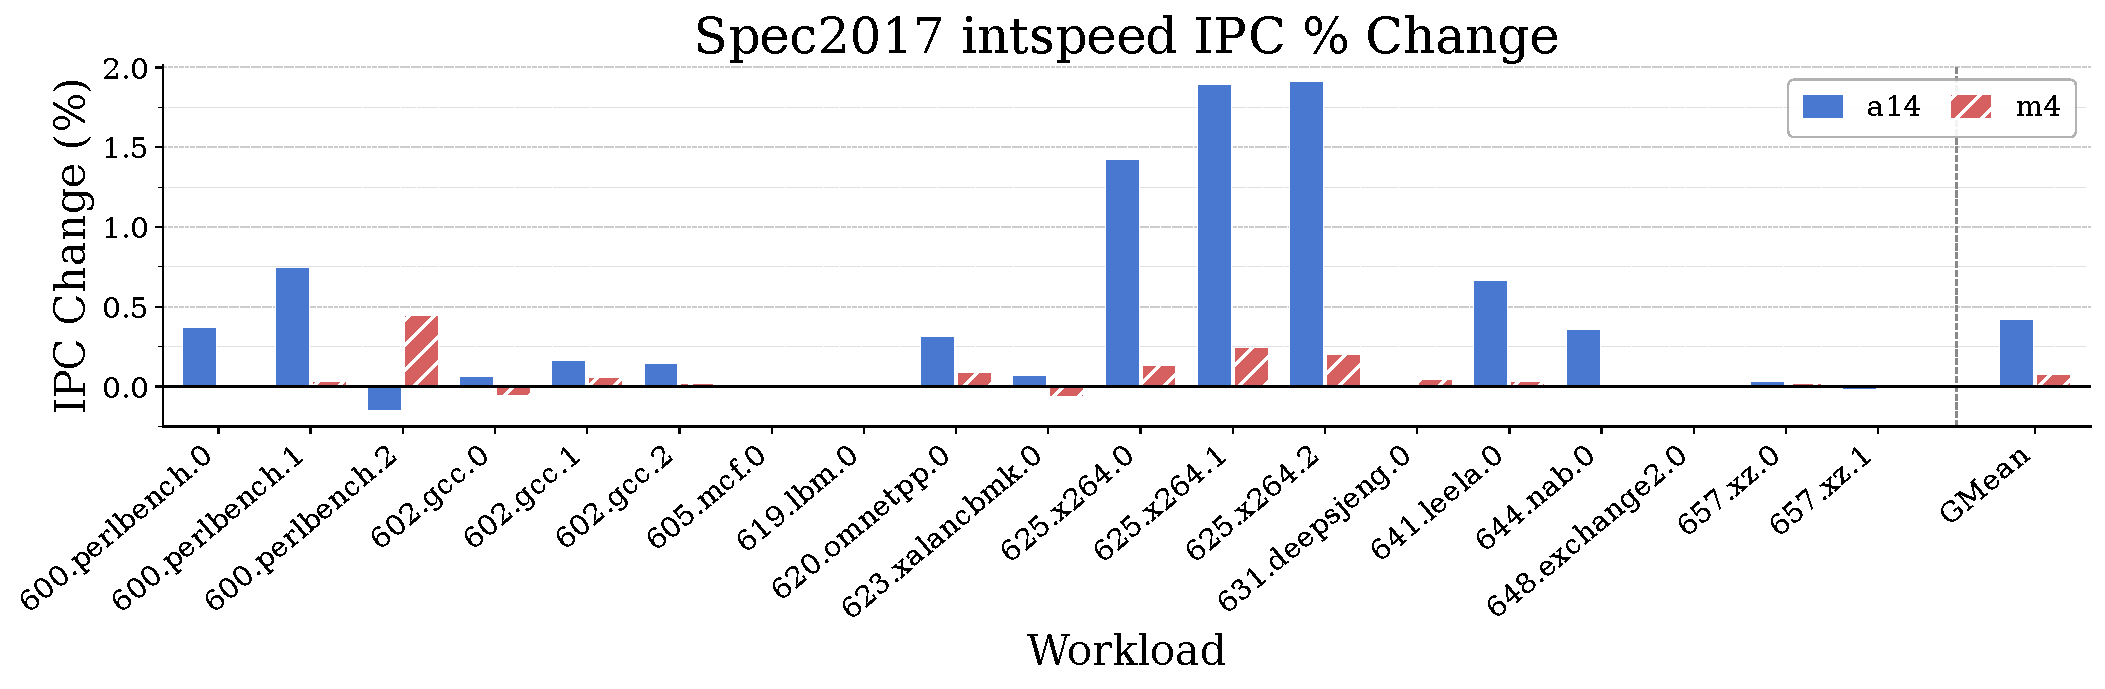
\includegraphics[width=\columnwidth,height=0.3\textheight, keepaspectratio]{figures/ipc_main.pdf}
\caption{IPC \% changes for each CPU model on each intspeed benchmark.}
\label{fig:ipc}
\end{figure}

Figure \ref{fig:ipc} shows the percent changes in IPC across Spec2017 intspeed for each core configuration. The gmean IPC gain ranges from 1.4\%, 0.7\% and 0\% as core size grows. This demonstrates our techniques ability to deliver zero-cost performance gains on area-constrained cores while still maintaining performance on larger cores with more sophisticated MDPs. Examining the gains in the best case (small core size), the IPC gains have an uneven spread across benchmarks, with some seeing large benefits and others next to none. This loosely correlates to the magnitude of false dependencies before and after seen in Figure \ref{fig:falsedeps}. The four largest gainers - $625.x264\_s$ inputs 1 and 2, $641.leela\_s$ and $620.omnetpp\_s$ - all exhibit relatively higher false dependencies per kilo-instruction in the base case, and see this cut down significantly by over 80\% when PND labels are used. As the core size increases to the medium configuration, most of these gains are diminished as the larger Store Set tables reduce the base number of hash collisions. A sensitivity analysis on the size of Store Sets on the small configuration results is shown in Section \ref{sec:storesetsize}.

%$600.perlbench\_s$ inputs 1 and 2 are outliers to this trend. They have the highest number of absolute false dependencies in the base case and also sees a significant reduction, yet only receives a modest IPC gain of around 1\% each. This is likely because the workloads are more frontend than backend bound, and so frequent frontend stalls mask most potential performance gains from issuing loads sooner. Whereas the average number of total icache misses across intspeed benchmarks is approximately 540k, $600.perlbench\_s$ inputs 1 and 2 observe 1.2M and 790k ichace misses respectively.

$620.omnetpp\_s$ exhibits more false dependencies per kilo-instruction in the medium core despite the larger Store Set size. This is likely because while it doesn't issue the most loads overall, it does have the highest number of dependent loads. Whereas the average across intspeed benchmarks is approximately 2 million dependent loads, $620.omnetpp\_s$ observes 6 million. This suggests due to the nature of the workload, a longer instruction window captures more dependencies which the larger Store Set tables cannot offset.

\begin{figure}[t]
  \centering
  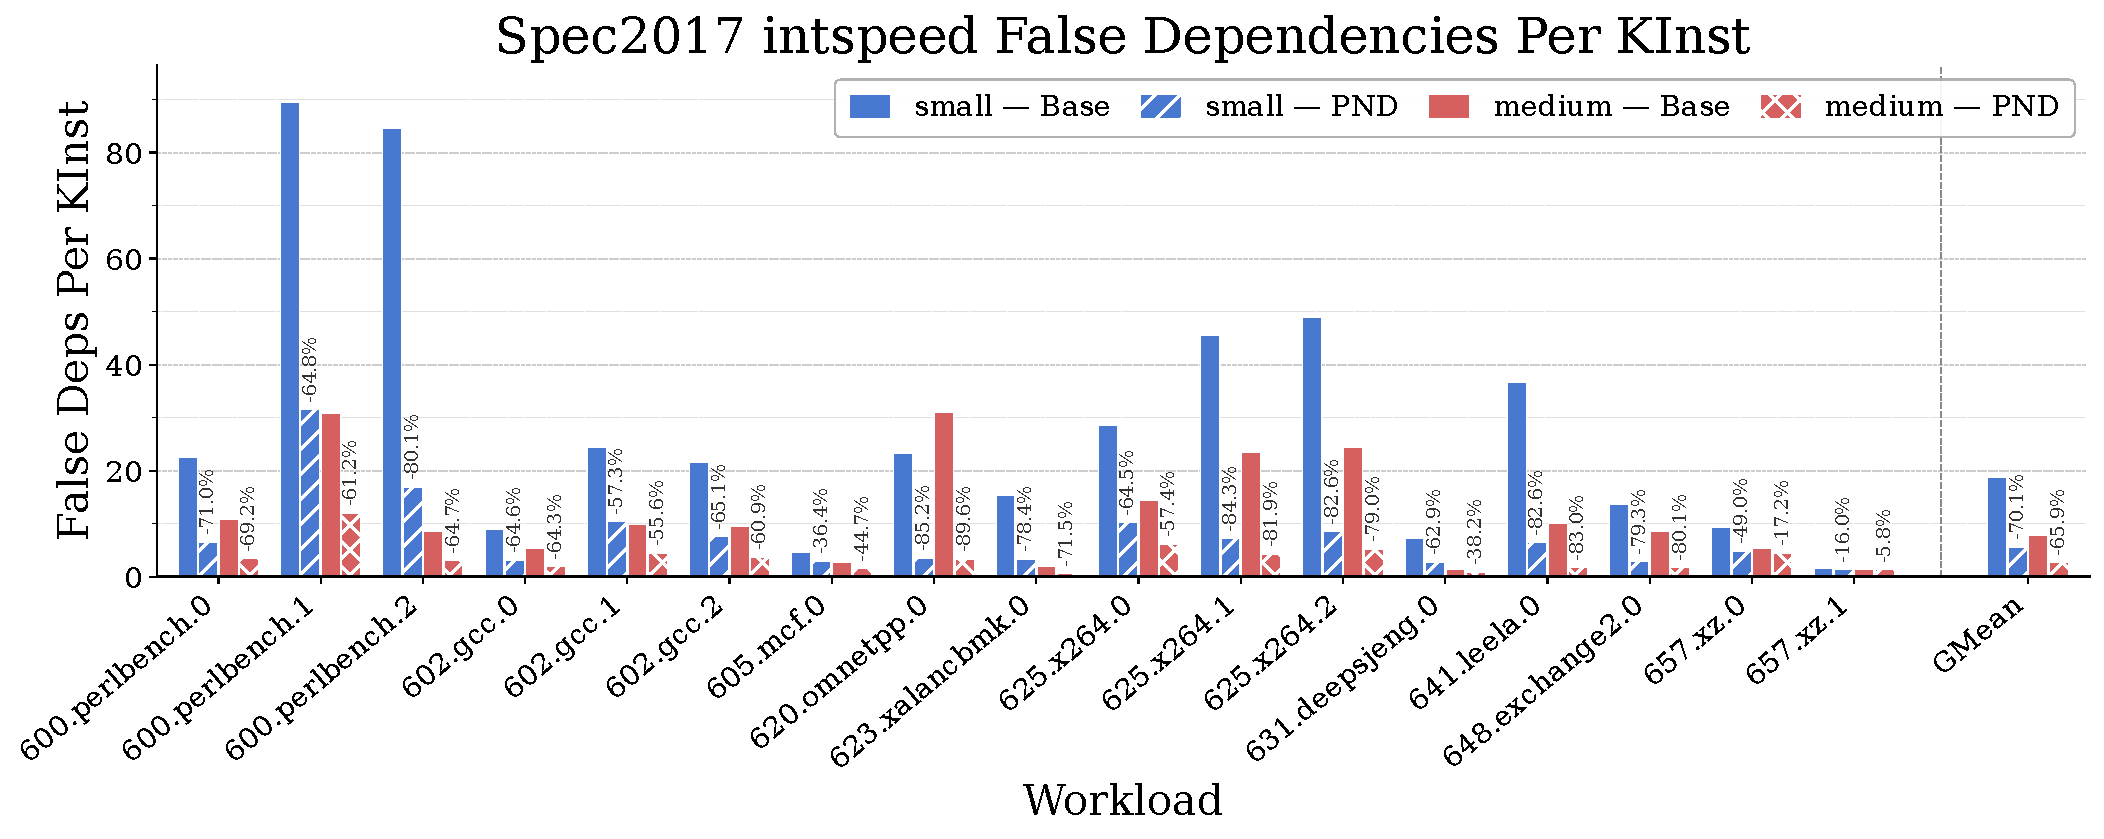
\includegraphics[width=\columnwidth,height=0.3\textheight, keepaspectratio]{figures/falsedeps_main.pdf}
\caption{Percent change of false dependencies.}
\label{fig:falsedeps}
\end{figure}

In select cases PND labels can lead to a performance regression, notably for input 2 of $600.perlbench\_s$. This is because loads have been mis-labelled from the train inputs and cause an increase in memory order violations on the test inputs, as seen in Figure \ref{fig:violations} for the medium core configuration. Although memory order violations are increased in all workloads, they're mostly offset by the reduction in false dependencies. It is also worth noting that violations are already very rare events, measured in mega-instructions rather than kilo-instructions, so even a 100\% increase can often still keep them in negligible ranges compared to the number of false dependencies. In input 2 of $600.perlbench\_s$ though the absolute number of violations is at it's highest, and so offsets any reductions in false dependencies (which as was also already discussed have more a limited impact in this workload).

%$620.omnetpp\_s$ sees the largest increase in violations yet maintains a performance gain for the medium configuration. This is possibly because it observes almost double the average intspeed dcache miss rate (4.3M vs 2.6M), leading to costly false dependencies that stall on stores long-to-resolve stores, but low penalty violations that occur during cache misses. 

The degree to which violations increase is controlled by the threshold value discussed in Section \ref{sec:method}. The optimal threshold may still provide a net performance gain while still causing small regressions in specific workloads, and a larger threshold could instead be chosen to ensure regressions never occur. They could be also mitigated by specialising the PGO technique to each benchmark rather than the processor.

\begin{figure}[t]
  \centering
  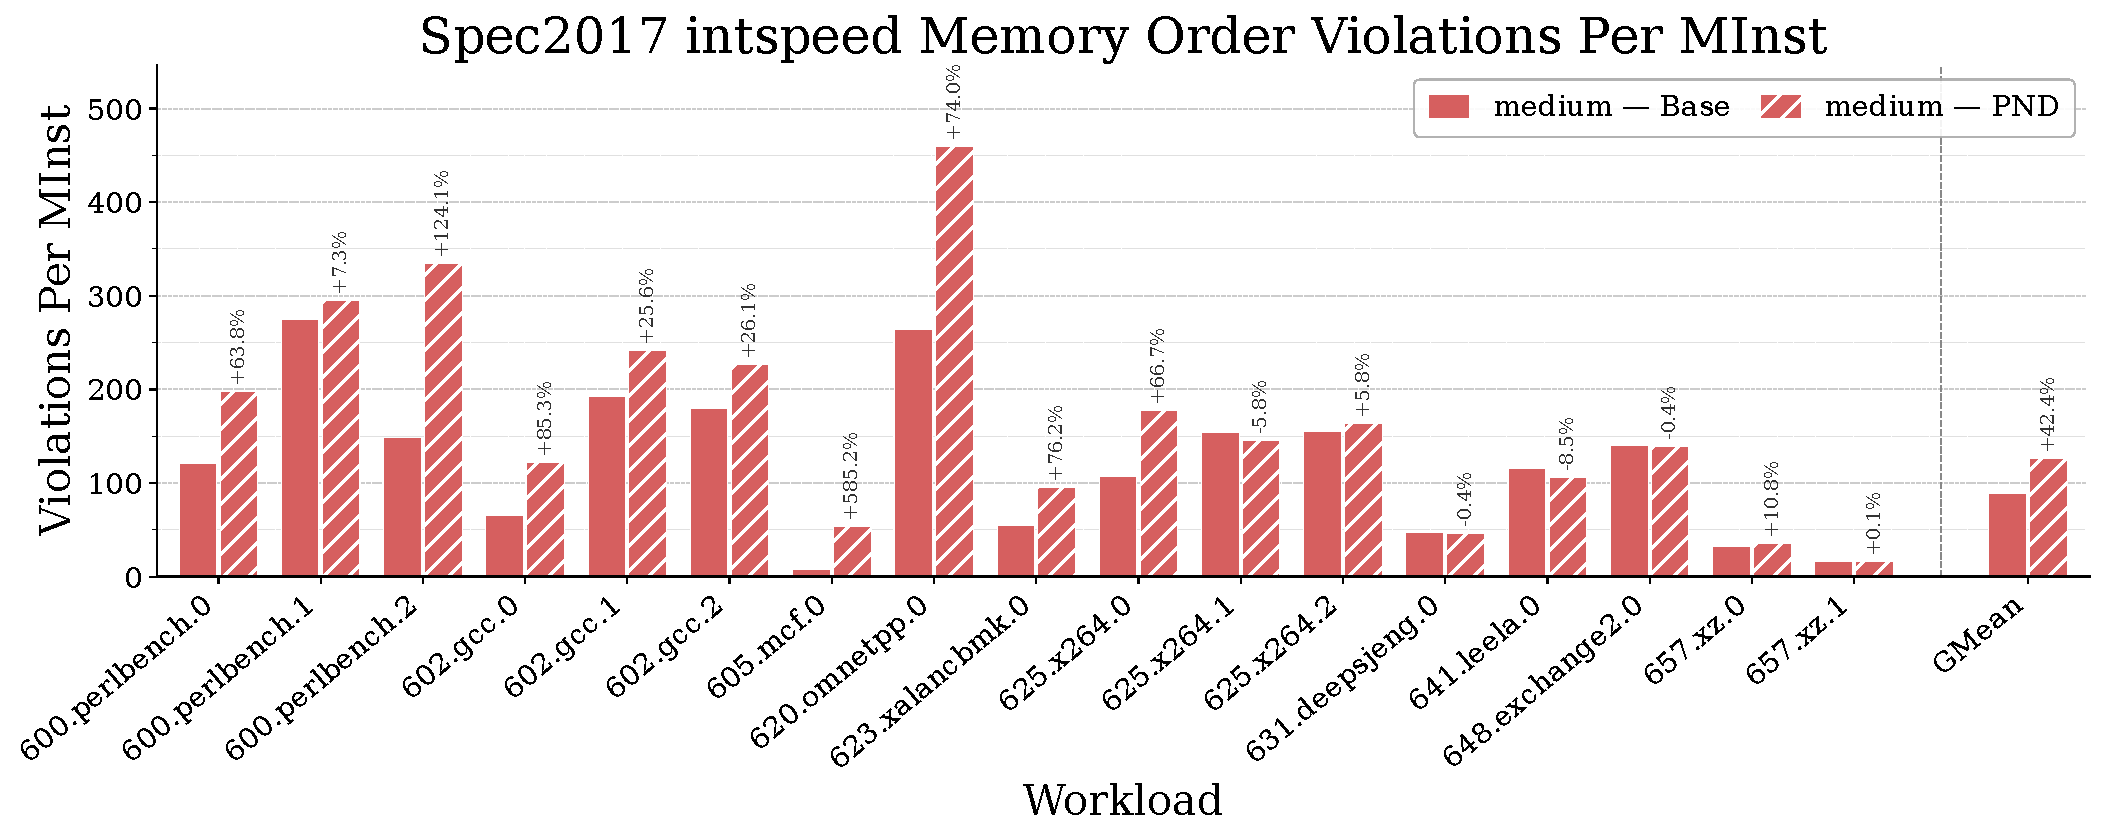
\includegraphics[width=\columnwidth,height=0.3\textheight, keepaspectratio]{figures/violations_medium.pdf}
\caption{Percent change of memory order violations. Values roughly equal between core sizes.}
\label{fig:violations}
\end{figure}

\subsection{Power}

- analyse power savings, correlated to lookup reduction. small core has small shift in MDP power, but total core power saving congruent to IPC gain, which is an opportuny to remind how the gains come at no area/power tradeoff.\\
- need large core results which have a larger MDP power saving, but next to no core change. can try and speculate how this offsets growing MDP power for the future\\
- need large core with big phast power savings which will hopefully nudge total core power a little more? not sure where to go with this section if it doesn't tho. 

\begin{figure}[t]
  \centering
  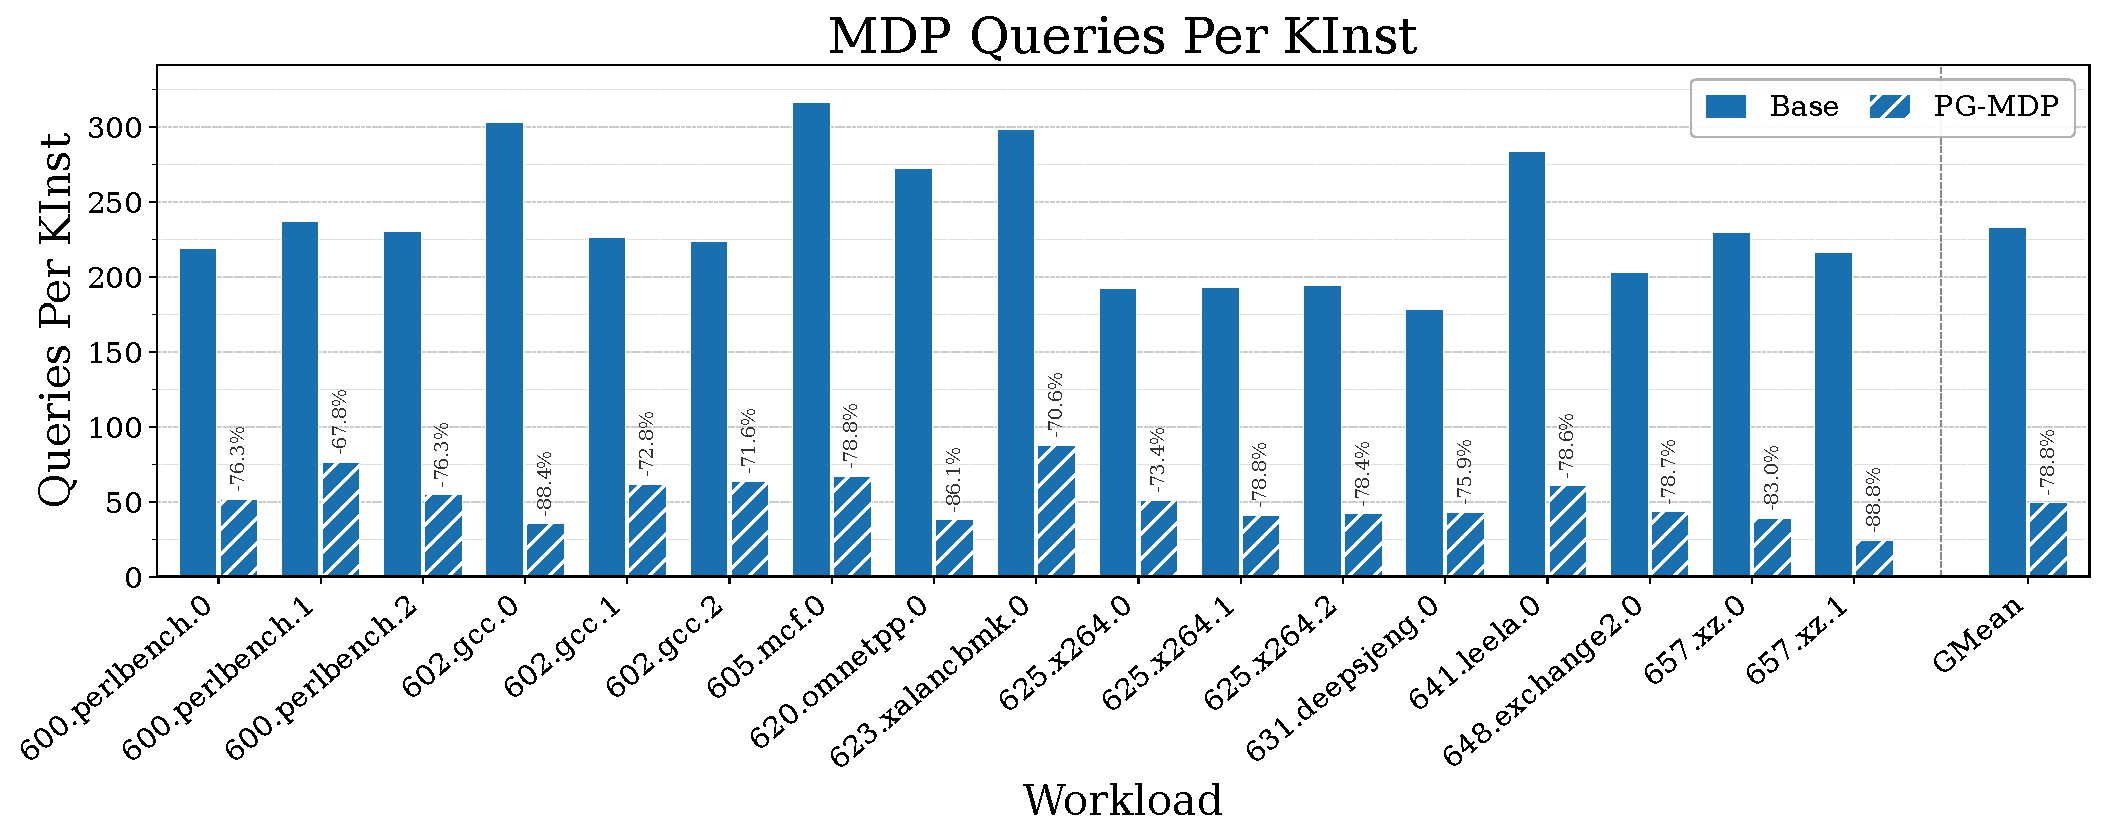
\includegraphics[width=\columnwidth,height=0.3\textheight, keepaspectratio]{figures/lookups_small.pdf}
\caption{Percent change of MDP queries. Values roughly equal between core sizes.}
\label{fig:lookups}
\end{figure}


\subsection{Read Port Impact Estimation}
Real processors have a limited number of read ports for each predictor component. If the memory dependence predictor has two ports, the processor can dispatch up to two memory operations per cycle. Gem5 does not model this behaviour by default, as it is a low-level detail that is difficult to represent accurately at the level of abstraction Gem5 simulates. Given the importance of this aspect to our proposed technique, we provide an estimation of the potential impact on IPC when read ports are limited. Each core configuration is assigned a number of read ports to the memory dependence predictor as listed in Table \ref{table:cpu-models}. The dispatch stage is modelled to block when the number of memory operations dispatched within a cycle exceeds the maximum number of read ports. This includes both loads and stores for XS Store Sets and only loads for PHAST. It is assumed that predictions always arrive within a single cycle for both XS Store Sets and PHAST, and so read port usage is reset to zero every cycle. This provides a rough estimation of the impact of predicted non-dependent loads on workloads with a high density of memory operations. For clarity, the number of MDP read ports does \textbf{not affect} any other results presented in this paper.\\

- insert results here

\subsection{Profile Analysis \& Threshold Sensitivity}

- need to generate profile from test input for this, will take a few days

\subsection{Store Set Table Size Sensitivity}
\label{sec:storesetsize}

As seen in Section \ref{sec:ipc}, the number of false dependencies falls sharply when increasing the Store Set table sizes along with core size. We present a sensitivity study for how gmean IPC improvement and base false dependencies in the small core configuration varies as both SSIT and LFST sizes grow. 

- graphs here\\

Figure \ref{fig:storesetsizefalsedeps} shows that the majority of false dependencies can be removed by growing the Store Set tables, and likewise Figure \ref{fig:storesetsizeipc} shows that the IPC gain diminishes along with this too. This demonstrates the main source of performance our technique offers is due to reducing hash collisions in the predictor tables, but without having to grow them.

Furthermore, we perform an iso-area comparison in the small core configuration between doubling the Store Set size verses growing the load queue by an equal number of bits. Whereas growing Store Sets provide an additional x\% gmean IPC, the larger load queue provides y\%. This suggests that Store Set hash collisions would not typically be eliminated in small processors by growing the predictor size.


\section{Threats to Validity}
- encoding space (cite cooperative memory disambig)\\
- cpu models (and gem5)\\
- intended for specific target compilation

\section{Future Work}
-per benchmark tuning \& JITs\\
-serverless workloads\\

\section{Conclusion}

%%%%%%% -- PAPER CONTENT ENDS -- %%%%%%%%

%%
%% The next two lines define the bibliography style to be used, and
%% the bibliography file.
\bibliographystyle{ACM-Reference-Format}
\bibliography{bibtex}

\end{document}
\endinput
%%
%% End of file `sample-sigconf.tex'.
